\documentclass[spec, och, otchet, hidelinks]{SCWorks}
% параметр - тип обучения - одно из значений:
%    spec     - специальность
%    bachelor - бакалавриат (по умолчанию)
%    master   - магистратура
% параметр - форма обучения - одно из значений:
%    och   - очное (по умолчанию)
%    zaoch - заочное
% параметр - тип работы - одно из значений:
%    otchet
%    referat    - реферат
%    coursework - курсовая работа (по умолчанию)
%    diploma    - дипломная работа
%    pract      - отчет по практике
%    pract      - отчет о научно-исследовательской работе
%    autoref    - автореферат выпускной работы
%    assignment - задание на выпускную квалификационную работу
%    review     - отзыв руководителя
%    critique   - рецензия на выпускную работу
% параметр - включение шрифта
%    times    - включение шрифта Times New Roman (если установлен)
%               по умолчанию выключен
\usepackage[T2A]{fontenc}
\usepackage[utf8]{inputenc}
\usepackage{graphicx}

\usepackage[sort,compress]{cite}
\usepackage{amsmath}
\usepackage{amssymb}
\usepackage{amsthm}
\usepackage{fancyvrb}
\usepackage{longtable}
\usepackage{array}
\usepackage[english,russian]{babel}
\usepackage{minted}
% Используется автором репозитория
%\usemintedstyle{xcode}
% Этот пакет включает в себя аналогичный Times New Roman шрифт.
% Необходим для успешной компиляции для UNIX-систем ввиду отсутствия TNR в нем.
% Можно использовать и для Windows.
\usepackage{tempora}


\usepackage[colorlinks=false]{hyperref}

\graphicspath{{figures/}}

\newcommand{\eqdef}{\stackrel {\rm def}{=}}

\usepackage{stackengine}
\newcommand\xrowht[2][0]{\addstackgap[.5\dimexpr#2\relax]{\vphantom{#1}}}

\newtheorem{lem}{Лемма}

% % При использовании biblatex вместо bibtex
%\usepackage[style=gost-numeric]{biblatex}
%\addbibresource{thesis.bib}

\begin{document}

% Кафедра (в родительном падеже)
\chair{математической кибернетики и компьютерных наук}

% Тема работы
\title{Аналого-цифровой преобразователь}

% Курс
\course{3}

% Группа
\group{331}

% Факультет (в родительном падеже) (по умолчанию "факультета КНиИТ")
%\department{факультета КНиИТ}

% Специальность/направление код - наименование
%\napravlenie{02.03.02 "--- Фундаментальная информатика и информационные технологии}
%\napravlenie{02.03.01 "--- Математическое обеспечение и администрирование информационных систем}
%\napravlenie{09.03.01 "--- Информатика и вычислительная техника}
%\napravlenie{09.03.04 "--- Программная инженерия}
\napravlenie{10.05.01 "--- Компьютерная безопасность}

% Для студентки. Для работы студента следующая команда не нужна.
%\studenttitle{Студентки}

% Фамилия, имя, отчество в родительном падеже
\author{Бородина Артёма Горовича}

% Заведующий кафедрой
\chtitle{доцент, к.\,ф.-м.\,н.} % степень, звание
\chname{С.\,В.\,Миронов}

%Научный руководитель (для реферата преподаватель проверяющий работу)
\satitle{аспирант}%, к.\,ф.-м.\,н.} %должность, степень, звание
\saname{А.\,А.\,Мартышкин}

% Руководитель практики от организации (только для практики,
% для остальных типов работ не используется)
\patitle{к.\,ф.-м.\,н., доцент}
\paname{Д.\,Ю.\,Петров}

% Семестр (только для практики, для остальных
% типов работ не используется)
\term{2}

% Наименование практики (только для практики, для остальных
% типов работ не используется)
\practtype{учебная}

% Продолжительность практики (количество недель) (только для практики,
% для остальных типов работ не используется)
\duration{2}

% Даты начала и окончания практики (только для практики, для остальных
% типов работ не используется)
\practStart{01.07.2016}
\practFinish{14.07.2016}

% Год выполнения отчета
\date{2022}

\maketitle

% Включение нумерации рисунков, формул и таблиц по разделам
% (по умолчанию - нумерация сквозная)
% (допускается оба вида нумерации)
%\secNumbering


\tableofcontents

% Раздел "Обозначения и сокращения". Может отсутствовать в работе
% \abbreviations
% \begin{description}
%     \item ... "--- ...
%     \item ... "--- ...
% \end{description}

% Раздел "Определения". Может отсутствовать в работе
%\definitions

% Раздел "Определения, обозначения и сокращения". Может отсутствовать в работе.
% Если присутствует, то заменяет собой разделы "Обозначения и сокращения" и "Определения"
%\defabbr


% Раздел "Введение"

\intro

Целью данной работы служит ознакомление с принципом работы и испытание интегрального 8-разрядного аналого-цифрового преобразователя.

\newpage

\section*{Задание 1.}
\addcontentsline{toc}{section}{Задание 1} 
Запустить лабораторный комплекс Labworks и среду МS10. Открыть файл \textbf{36.4.ms10}, размещенный в папке \textbf{Circuit Design Suitе 10.0} среды 
МS10, или собрать на рабочем поле среды MS10 схему для испытания \textit{аналого-цифрового преобразователя} с ЦАП и установить в диалоговых окнах 
компонентов их параметры или режимы работы. \textbf{Скопировать} схему в отчет.

\begin{figure}[h]
	\center{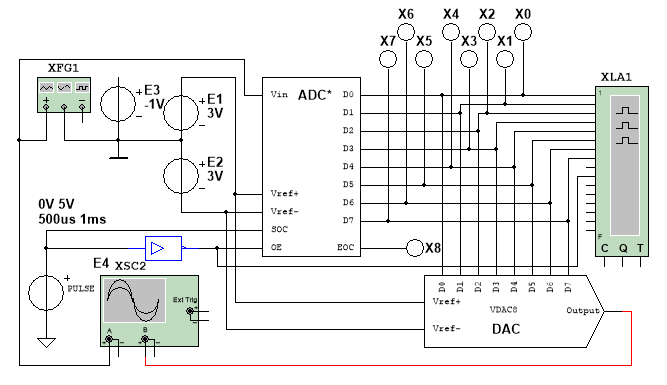
\includegraphics{scheme_task_one.png}}
	\caption{Схема аналого-цифрового преобразователя.}
\end{figure}

\newpage

\section*{Задание 2.}
\addcontentsline{toc}{section}{Задание 2}

\textbf{Исследовать} точность преобразования АЦП уровней входного напряжения $u_\text{вх}$ в цифровой код с помощью пробников \textbf{Х0, $\dots$, Х7}, 
логического анализатора \textbf{ХLA1}, а также ЦАП и осциллографа \textbf{XSC1}.
\par С этой целью:

• временно \textbf{удалить} провод 1 и подключить вход \textbf{Vin} АЦП к положительному полюсу источника постоянного напряжения \textbf{Е3};

\begin{figure}[h]
	\center{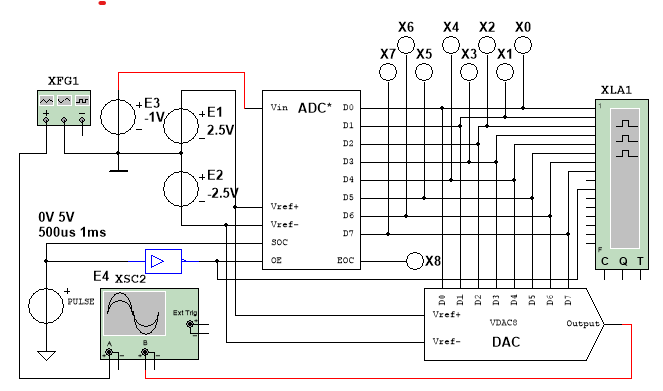
\includegraphics{new_configuration.png}}
	\caption{Подключение входа \textbf{Vin} АЦП к положительному полюсу источника постоянного напряжения \textbf{E3} и изменение ЭДС генераторов.}
\end{figure}

• составить таблицу, в первый столбец которой записать уровни напряжения: $ u_\text{вх} = 0,1; \, 0,2; \, 0,5; \, 1,0; \, 1,5; \, 2,0; \, 2,4; \, 
-0,5; \, -1,0; \, -2,0 $ В, поочередно задаваемые в диалоговом окне генератора \textbf{Е3}; 

• \textbf{установить} в диалоговых окнах генераторов \textbf{Е1} и \textbf{Е2} ЭДС $E_1$ = 2,5 В, и $E_2$ = –2,5 В;

• \textbf{запустить} программу моделирования АЦП и \textbf{заносить} в составленную таблицу значения напряжения $u_\text{вых(цап)}$ с выхода ЦАП, 
измеряемые на экране осциллографа с помощью визирной линии; двоичный эквивалент $D_{(2)}$ преобразуемого напряжения, определяемый по свечению пробников 
\textbf{Х7, \dots, Х0}; шестнадцатеричный код $D_{(16)}$, считываемый с дисплея анализатора \textbf{XLA1};

• получаемые с выхода АЦП десятичные инверсные сигналы $D_\text{(10)инв}$ пересчитать на неинверсные $D_{(10)}$ по выражению $D_{(10)} = D_\text{(10)инв} 
- 128$ и занести в соответствующие столбцы таблицы;

• расчетные десятичные эквиваленты $D_\text{(10)расч}$ двоичного кода $D_{(2)}$ на выходе АЦП при заданном значении входного напряжения $u_\text{вх}$ 
\textbf{определить} по формуле $D_\text{(10)расч} = 256u_\text{вх} /(E_1+ |-E_2|)$ и занести во второй справа столбец таблицы;

• \textbf{рассчитать} погрешности измерения напряжения по выражению $\Delta U\% = 100(u_\text{вых(цап)} - u_\text{вх})/u_\text{вх} $ и занести в правый 
столбец таблицы.

\begin{table}[h!]
	\centering
	\captionsetup{justification=centering}
	\begin{tabular}{|c|c|c|c|c|c|c|c|}
		\hline\xrowht[()]{10pt}
		$u_\text{вх},$ В & $u_\text{вых(цап)},$ В &  $D_\text{(2)}$ & $D_\text{(16)}$ & $D_\text{(10)инв}$ & $D_\text{(10)}$ & $D_\text{(10)расч}$ & $\Delta U \%$ \\
		\hline\xrowht[()]{10pt}
		0.1 & 0.0938 & 10000101 & 85 & 133 & 5 & 5.12 & 6.25 \\
		\hline\xrowht[()]{10pt}
		0.2 & 0.2042 & 10001010 & 8A & 138 & 10 & 10.24 & 2.1 \\
		\hline\xrowht[()]{10pt}
		0.5 & 0.5158 & 10011010 & 9A & 154 & 26 & 25.6 & 3.12 \\ 
		\hline\xrowht[()]{10pt}
		1 & 0.9645 & 10110011 & B3 & 179 & 51 & 51.2 & 3.56 \\
		\hline\xrowht[()]{10pt}
		1.5 & 1.5042 & 11001101 & CD & 205 & 77 & 76.8 & 0.28 \\
		\hline\xrowht[()]{10pt}
		2 & 2.017 & 11100110 & E6 & 230 & 102 & 102.4 & 0.85 \\
		\hline\xrowht[()]{10pt}
		2.4 & 2.393 & 11111011 & FB & 251 & 123 & 122.88 & 0.3 \\
		\hline\xrowht[()]{10pt}
		-0.5 & -0.5042 & 01100110 & 66 & 102 & -26 & -25.6 & 1.5 \\
		\hline\xrowht[()]{10pt}
		-1 & -0.9844 & 01001101 & 4D & 77 & -51 & -51.2 & 3.56 \\
		\hline\xrowht[()]{10pt}
		-2 & -2.009 & 00011010 & 1A & 25 & -102 & -102.5 & 0.46 \\
		\hline
	\end{tabular}
	\caption{Значения выходного напряжения $u_\text{вых.}$ ЦАП.}
\end{table}


\section*{Задание 3.}
\addcontentsline{toc}{section}{Задание 3}

\textbf{Исследовать} процесс преобразования входного напряжения треугольной формы в цифровые коды, а затем с помощью ЦАП – в ступенчатое напряжение, 
аппроксимирующее напряжение $u_\text{вх}$. Для этого:

• \textbf{удалить} провод, соединяющий выход генератора \textbf{Е3} с входом \textbf{Vin} АЦП, и \textbf{восстановить} провод 1, соединяющий выход «+» 
функционального генератора \textbf{XFG1} с входом Vin АЦП;

• \textbf{установить} параметры генератора \textbf{XFG1}: напряжение треугольной формы со скважностью $N$ = 99 и амплитудой 1 В и его частоту 
$f_\text{г}$ = 50 Гц;

\begin{figure}[h]
	\center{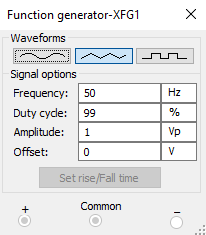
\includegraphics{gen_params.png}}
	\caption{Установка параметров генератора.}
\end{figure}

• \textbf{запустить} программу моделирования АЦП;

\newpage

• \textbf{получить} и \textbf{скопировать} в отчет осциллограмму входного напряжения $u_\text{вх}$, осциллограмму ступенчатого напряжения 
$u_\text{вых(цап)}$ с выхода ЦАП и временные диаграммы сигналов с выходов \textbf{D0, \dots, D7} АЦП, поступающих на входы логического анализатора 
\textbf{XLA1} и являющихся двоичными эквивалентами дискретных отсчетов $ u_\text{вх} (k \Delta t) $ входного напряжения; 

\begin{figure}[h]
	\center{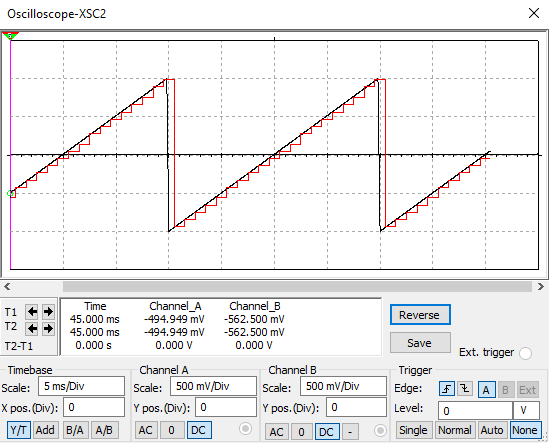
\includegraphics[scale=0.75]{oscillo.png}}
	\caption{Осциллограмма входного напряжения.}
\end{figure}

\begin{figure}[h!]
	\center{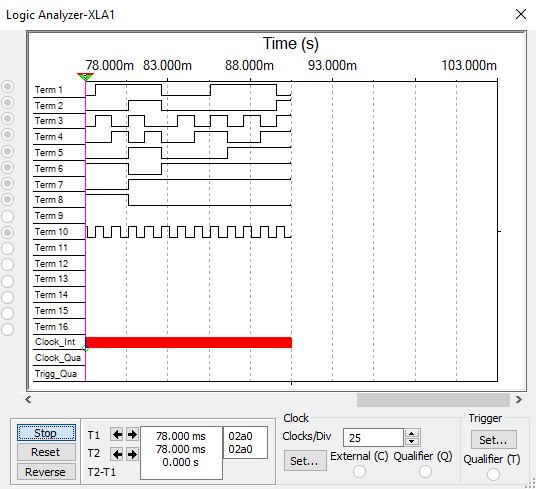
\includegraphics[scale=0.75]{logic_analyzer.png}}
	\caption{Временные диаграммы сигналов.}
\end{figure}

\newpage

\section*{Задание 4.}
\addcontentsline{toc}{section}{Задание 4}

\textbf{Исследовать} процесс преобразования АЦП входного синусоидального напряжения в цифровые коды, а затем с помощью ЦАП – в ступенчатое напряжение.

\par С этой целью:

• \textbf{щелкнуть мышью} на кнопке «Синусоидальное напряжение» генератора \textbf{ХFG1} и \textbf{установить} частоту напряжения $f_\text{г}$ = 25 Гц, 
а затем, при остановке моделирования, $f_\text{г}$ = 5 Гц с изменением времени развертки лучей осциллографа с 10 мс/дел на 50 мс/дел. \textbf{Сместить} 
вверх на 0,6 деления осциллограмму входного напряжения $u_\text{вх}$;

\begin{figure}[h]
	\center{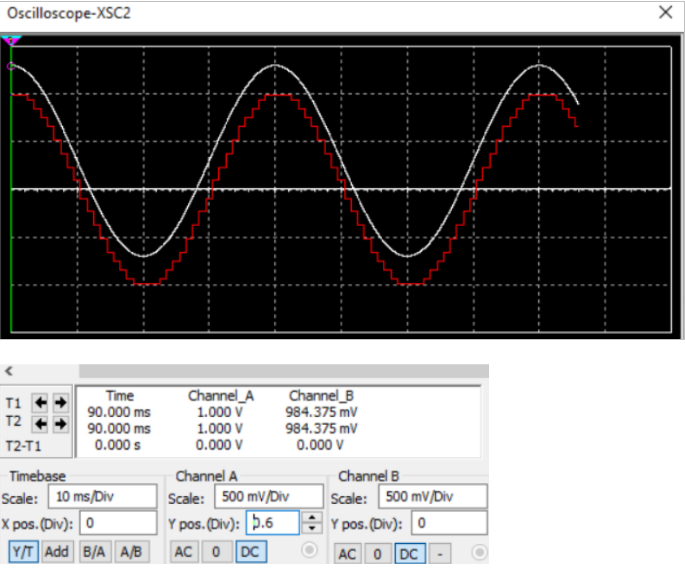
\includegraphics[scale=0.7]{oscillo_sin.png}}
	\caption{Синусоидальное напряжение.}
\end{figure}

\newpage

\section*{Тестовые задания.}
\addcontentsline{toc}{section}{Тестовые задания}

\par 1. Укажите \textbf{назначение} АЦП: \textbf{для преобразования постоянного напряжения, заданного на тактовом интервале, в двоичный код};

\par 2. Укажите \textbf{формулу Котельникова}, с помощью которой определяют шаг дискретизации $\Delta t$ аналогового сигнала ($f_m$ – максимальная 
частота спектра аналогового сигнала; $t_\text{вх}$ – длительность аналогового сигнала; $N$ – число уровней квантования): $\Delta t \leq 1 / 2f_m$;

\par 3. Определите понятие «\textbf{абсолютная разрешающая способность}» АЦП: \textbf{это среднее значение минимального изменения входного сигнала, 
	обусловливающего увеличение или уменьшение выходного кода на единицу};

\par 4. Укажите, можно ли подавать на входы $V_{ref^{+}}$ и $V_{ref^{-}}$ АЦП \textbf{разные} (по модулю) \textbf{напряжения}: \textbf{да};

\par 5. Укажите, можно ли \textbf{свести к нулю} погрешность квантования аналогового сигнала посредством выбора параметров устройства, например за счет 
увеличения разрядности АЦП: \textbf{нет};

\par 6. Укажите, какую погрешность квантования имеет 8-разрядный АЦП при напряжениях на входах $V_{ref^{+}}$ = 2 В, $V_{ref^{–}}$ = 0 и отсчете входного 
напряжения $u_\text{вх}(k\Delta t)$ = 1 В: $\pm 3,9$ мВ;

\par 7. Укажите \textbf{десятичный эквивалент} двоичного кода на выходе 8-разрядного АЦП, если опорные напряжения $V_{ref^{+}}$ = 2 В, $V_{ref^{–}}$ 
= –2 В, а входное напряжение $u_\text{вх}$ = 0,5 В: \textbf{32};

\par 8. Выберите из приведенных ниже значений минимально необходимые \textbf{значения опорных напряжений} $\pm V_{ref}$ для преобразования синусоидального 
напряжения $u_\text{вх}(t) = 1,41\sin \omega t$: $\pm 2$ В;

\par 9. Укажите значение расчетного шестнадцатеричного кода 16-разрядного АЦП, если на его вход подано напряжение $u_\text{вх}(k \Delta t)$ = 0,25 В 
при $ \pm V_{ref} = \pm 2 В$: \textbf{1000};

\par 10. Укажите \textbf{выражение}, с помощью которого определяют десятичный эквивалент двоичного кода на выходе 14-разрядного АЦП: 
$D = 4096u_\text{вх} / (V_{ref^{+}} + |-V_{ref^{-}}|)$;

\par 11. Укажите, как изменится \textbf{выходной код} АЦП при неизменном входном $u_\text{вх}$ и опорных напряжениях $V_{ref}^{+}$ = 2 В и $V_{ref}^{–}$
 = –2 В, если установить $V_{ref}^{–}$ = 0: \textbf{его значение уменьшится в два раза};

\par 12. Укажите характер изменения \textbf{общей погрешности} преобразования входного сигнала при увеличении разрядности АЦП: \textbf{погрешность преобразования уменьшится};

\par 13. Укажите перспективные \textbf{направления} развития АЦП: \textbf{повышение быстродействия основных узлов АЦП, в частности компараторов; применение
стабилизированных источников опорного напряжения; использование микропроцессоров в преобразователях};

\par 14. Укажите, какие \textbf{операции} необходимо выполнить при аналого-цифровом преобразовании: \textbf{дискретизацию по времени аналогового сигнала, 
квантования по уровню его отсчётов и кодирование квантованных уровней};

\par 15. Укажите, обладает ли способ последовательного счета аналого-цифрового преоб-
разования наибольшим быстродействием: \textbf{да}.

\newpage

\conclusion

В ходе данной лабораторной работы мы ознакомились с принципом работы 8-рязрядного аналого-цифрового преобразователя и испытали его на практике.

\end{document}